\documentclass[11pt,a4paper]{article}
\usepackage[spanish]{babel}					% Utilizar español
\usepackage[utf8]{inputenc}					% Caracteres UTF-8
\usepackage{graphicx}						% Imagenes
\usepackage[hidelinks]{hyperref}			% Poner enlaces sin marcarlos en rojo
\usepackage{fancyhdr}						% Modificar encabezados y pies de pagina
\usepackage{float}							% Insertar figuras
\usepackage[textwidth=390pt]{geometry}		% Anchura de la pagina
\usepackage[nottoc]{tocbibind}				% Referencias (no incluir num pagina indice en Indice)
\usepackage{enumitem}

% Configuracion de encabezados y pies de pagina
\pagestyle{fancy}
\lhead{Vladislav Nikolov Vasilev}
\rhead{Asignatura}
\lfoot{Grado en Ingeniería Informática}
\cfoot{}
\rfoot{\thepage}
\renewcommand{\headrulewidth}{0.4pt}		% Linea cabeza de pagina
\renewcommand{\footrulewidth}{0.4pt}		% Linea pie de pagina


\newcommand{\answer}{\noindent\textbf{Solución}}


\begin{document}
\pagenumbering{gobble}

% Pagina de titulo
\begin{titlepage}

\begin{minipage}{\textwidth}

\centering

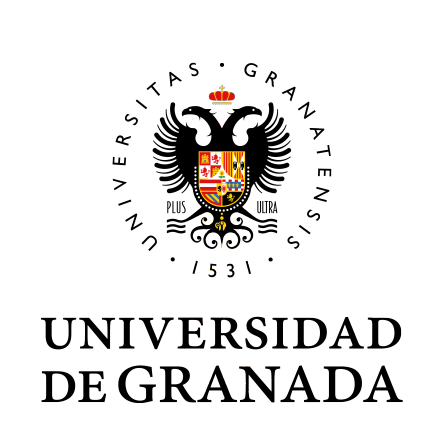
\includegraphics[scale=0.5]{img/ugr.png}\\

\textsc{\Large Aprendizaje Automático\\[0.2cm]}
\textsc{GRADO EN INGENIERÍA INFORMÁTICA}\\[1cm]

\noindent\rule[-1ex]{\textwidth}{1pt}\\[1.5ex]
\textsc{{\Huge TRABAJO 1\\[0.5ex]}}
\textsc{{\Large Cuestiones de Teoría\\}}
\noindent\rule[-1ex]{\textwidth}{2pt}\\[3.5ex]

\end{minipage}

\vspace{0.5cm}

\begin{minipage}{\textwidth}

\centering

\textbf{Autor}\\ {Vladislav Nikolov Vasilev}\\[2.5ex]
\textbf{Rama}\\ {Computación y Sistemas Inteligentes}\\[2.5ex]
\vspace{0.3cm}


\includegraphics[scale=0.3]{img/etsiit.jpeg}

\vspace{0.7cm}
\textsc{Escuela Técnica Superior de Ingenierías Informática y de Telecomunicación}\\
\vspace{1cm}
\textsc{Curso 2018-2019}
\end{minipage}
\end{titlepage}

\pagenumbering{arabic}
\tableofcontents
\thispagestyle{empty}				% No usar estilo en la pagina de indice

\newpage

\setlength{\parskip}{1em}

\section*{Ejercicio 1}
\addcontentsline{toc}{section}{Ejercicio 1}

\noindent Identificar, para cada una de las siguientes tareas, cuál es el problema, qué tipo de aprendizaje es el adecuado
(supervisado, no supervisado, por refuerzo) y los elementos de aprendizaje $(\mathcal{X} , f, \mathcal{Y})$ que deberíamos
usar en cada caso. Si una tarea se ajusta a más de un tipo, explicar como y describir los elementos para cada tipo.

\begin{enumerate}[label=\textit{\alph*})]
	\item Clasificación automática de cartas por distrito postal.
\end{enumerate}

\answer

El problema en este caso consiste en clasificar cartas por distrito postal.

\begin{enumerate}[resume,label=\textit{\alph*})]
	\item Decidir si un determinado índice del mercado de valores subirá o bajará dentro de un período de tiempo fijado.
\end{enumerate}

\answer

El problema en este caso consiste en predecir o decidir a partir de unos datos de entrada una clase (la de si subirá o bajará
el índice de mercado). Por tanto este problema se puede ver como una clasificación binaria $(0, 1)$ o $(-1, 1)$.

En el caso de los datos de entrada $\mathcal{X}$ podríamos utilizar valores del mercado y el tiempo. En el caso de los datos
de salida o etiquetas $\mathcal{Y}$ podríamos tener las etiquetas $(-1, 1)$, siendo $-1$ el caso de bajar el índice y $1$ el
de subir. Y por último, $f$ sería una función que relacione a $\mathcal{X}$ y a $\mathcal{Y}$ tal que $f: \; \mathcal{X}
\mapsto \mathcal{Y}$, como por ejemplo el la función signo, usada en el algoritmo PLA.

\begin{enumerate}[resume,label=\textit{\alph*})]
	\item Hacer que un dron sea capaz de rodear un obstáculo.
\end{enumerate}

\answer

El problema en este caso es hacer que un dron aprenda a esquivar un obstáculo rodeándolo. Como el objetivo no es clasificar
ninguna información, ni predecir ningún valor real ni buscar características o patrones en los datos, parece que el tipo
de aprendizaje más adecuado es el aprendizaje por refuerzo. Esto se podría hacer mediante un simulador en un ordenador, donde
se representaría el espacio donde se quiere entrenar al dron. Una vez entrenado en este simulador, se podría transferir todo
lo aprendido al dron y ver cómo se desempeña.

Como tal, el aprendizaje por refuerzo no tendría ni entradas $\mathcal{X}$, ni etiquetas de salida $\mathcal{Y}$ ni una
función $f$ para el aprendizaje, pero sí que tendría otra información que se correspondería con un Proceso de Decisión de
Markov (MDP), como por ejemplo un conjunto de estados, acciones, probabilidades de transicionar de un estado a otro, una
recompensa por transicionar de estado, etc.

\begin{enumerate}[resume,label=\textit{\alph*})]
	\item Dada una colección de fotos de perros, posiblemente de distintas razas, establecer
	cuántas razas distintas hay representadas en la colección.
\end{enumerate}

\answer

En este caso el problema consiste en encontrar patrones o características que permitan agrupar los datos (agrupar los perros
según su raza, para saber cuántas hay). Por tanto, al no saber a priori cómo se clasifican los datos, el aprendizaje no
supervisado sería la mejor opción para descubrir como se agrupan éstos.

En este caso, $\mathcal{X}$ son los datos de los que dispondríamos (las fotos de los perros), $\mathcal{Y}$ sería desconocido
ya que no sabemos qué clases hay (no sabemos las razas de perros) y $f$ sería una función de distribución condicional que se
quiere aprender con tal de intentar agrupar los datos.

\section*{Ejercicio 2}
\addcontentsline{toc}{section}{Ejercicio 2}

\noindent ¿Cuáles de los siguientes problemas son más adecuados para una aproximación por aprendizaje y cuáles más adecuados
para una aproximación por diseño? Justificar la decisión.

\begin{enumerate}[label=\textit{\alph*})]
	\item Determinar si un vertebrado es mamífero, reptil, ave, anfibio o pez.
\end{enumerate}

\begin{enumerate}[resume,label=\textit{\alph*})]
	\item Determinar si se debe aplicar una campaña de vacunación contra una enfermedad.
\end{enumerate}

\begin{enumerate}[resume,label=\textit{\alph*})]
	\item Determinar perfiles de consumidor en una cadena de supermercados.
\end{enumerate}

\begin{enumerate}[resume,label=\textit{\alph*})]
	\item Determinar el estado anímico de una persona a partir de una foto de su cara.
\end{enumerate}

\begin{enumerate}[resume,label=\textit{\alph*})]
	\item Determinar el ciclo óptimo para las luces de los semáforos en un cruce con mucho tráfico.
\end{enumerate}



\newpage

\begin{thebibliography}{5}

\bibitem{nombre-referencia}
Texto referencia
\\\url{https://url.referencia.com}

\end{thebibliography}

\end{document}

